% Options for packages loaded elsewhere
\PassOptionsToPackage{unicode}{hyperref}
\PassOptionsToPackage{hyphens}{url}
\PassOptionsToPackage{dvipsnames,svgnames,x11names}{xcolor}
%
\documentclass[
  10pt,
  ignorenonframetext,
]{beamer}
\usepackage{pgfpages}
\setbeamertemplate{caption}[numbered]
\setbeamertemplate{caption label separator}{: }
\setbeamercolor{caption name}{fg=normal text.fg}
\beamertemplatenavigationsymbolsempty
% Prevent slide breaks in the middle of a paragraph
\widowpenalties 1 10000
\raggedbottom
\setbeamertemplate{part page}{
  \centering
  \begin{beamercolorbox}[sep=16pt,center]{part title}
    \usebeamerfont{part title}\insertpart\par
  \end{beamercolorbox}
}
\setbeamertemplate{section page}{
  \centering
  \begin{beamercolorbox}[sep=12pt,center]{part title}
    \usebeamerfont{section title}\insertsection\par
  \end{beamercolorbox}
}
\setbeamertemplate{subsection page}{
  \centering
  \begin{beamercolorbox}[sep=8pt,center]{part title}
    \usebeamerfont{subsection title}\insertsubsection\par
  \end{beamercolorbox}
}
\AtBeginPart{
  \frame{\partpage}
}
\AtBeginSection{
  \ifbibliography
  \else
    \frame{\sectionpage}
  \fi
}
\AtBeginSubsection{
  \frame{\subsectionpage}
}
\usepackage{amsmath,amssymb}
\usepackage{iftex}
\ifPDFTeX
  \usepackage[T1]{fontenc}
  \usepackage[utf8]{inputenc}
  \usepackage{textcomp} % provide euro and other symbols
\else % if luatex or xetex
  \usepackage{unicode-math} % this also loads fontspec
  \defaultfontfeatures{Scale=MatchLowercase}
  \defaultfontfeatures[\rmfamily]{Ligatures=TeX,Scale=1}
\fi
\usepackage{lmodern}
\usetheme[]{metropolis}
\ifPDFTeX\else
  % xetex/luatex font selection
\fi
% Use upquote if available, for straight quotes in verbatim environments
\IfFileExists{upquote.sty}{\usepackage{upquote}}{}
\IfFileExists{microtype.sty}{% use microtype if available
  \usepackage[]{microtype}
  \UseMicrotypeSet[protrusion]{basicmath} % disable protrusion for tt fonts
}{}
\makeatletter
\@ifundefined{KOMAClassName}{% if non-KOMA class
  \IfFileExists{parskip.sty}{%
    \usepackage{parskip}
  }{% else
    \setlength{\parindent}{0pt}
    \setlength{\parskip}{6pt plus 2pt minus 1pt}}
}{% if KOMA class
  \KOMAoptions{parskip=half}}
\makeatother
\usepackage{xcolor}
\newif\ifbibliography
\usepackage{listings}
\newcommand{\passthrough}[1]{#1}
\lstset{defaultdialect=[5.3]Lua}
\lstset{defaultdialect=[x86masm]Assembler}
\usepackage{graphicx}
\makeatletter
\def\maxwidth{\ifdim\Gin@nat@width>\linewidth\linewidth\else\Gin@nat@width\fi}
\def\maxheight{\ifdim\Gin@nat@height>\textheight\textheight\else\Gin@nat@height\fi}
\makeatother
% Scale images if necessary, so that they will not overflow the page
% margins by default, and it is still possible to overwrite the defaults
% using explicit options in \includegraphics[width, height, ...]{}
\setkeys{Gin}{width=\maxwidth,height=\maxheight,keepaspectratio}
% Set default figure placement to htbp
\makeatletter
\def\fps@figure{htbp}
\makeatother
\setlength{\emergencystretch}{3em} % prevent overfull lines
\providecommand{\tightlist}{%
  \setlength{\itemsep}{0pt}\setlength{\parskip}{0pt}}
\setcounter{secnumdepth}{-\maxdimen} % remove section numbering
\ifLuaTeX
\usepackage[bidi=basic]{babel}
\else
\usepackage[bidi=default]{babel}
\fi
\babelprovide[main,import]{american}
% get rid of language-specific shorthands (see #6817):
\let\LanguageShortHands\languageshorthands
\def\languageshorthands#1{}
\usepackage{fancyhdr}
\pagestyle{fancy}
\usepackage{setspace}
\usepackage{graphicx}
\usepackage{amsfonts}
\usepackage{amssymb}
\usepackage{amsmath}
\usepackage{minted}
\ifLuaTeX
  \usepackage{selnolig}  % disable illegal ligatures
\fi
\IfFileExists{bookmark.sty}{\usepackage{bookmark}}{\usepackage{hyperref}}
\IfFileExists{xurl.sty}{\usepackage{xurl}}{} % add URL line breaks if available
\urlstyle{same}
\hypersetup{
  pdftitle={Understanding Memory Management},
  pdfauthor={Dipesh Kafle},
  pdflang={en-US},
  colorlinks=true,
  linkcolor={blue},
  filecolor={Maroon},
  citecolor={Blue},
  urlcolor={red},
  pdfcreator={LaTeX via pandoc}}

\title{Understanding Memory Management}
\author{Dipesh Kafle}
\date{}

\begin{document}
\frame{\titlepage}

\hypertarget{prerequisites}{%
\section{Prerequisites}\label{prerequisites}}

\begin{frame}{Memory Layout}
\protect\hypertarget{memory-layout}{}
\begin{columns}[T]
\begin{column}{0.1\textwidth}
\end{column}

\begin{column}{0.9\textwidth}
\pause

\begin{figure}
\centering
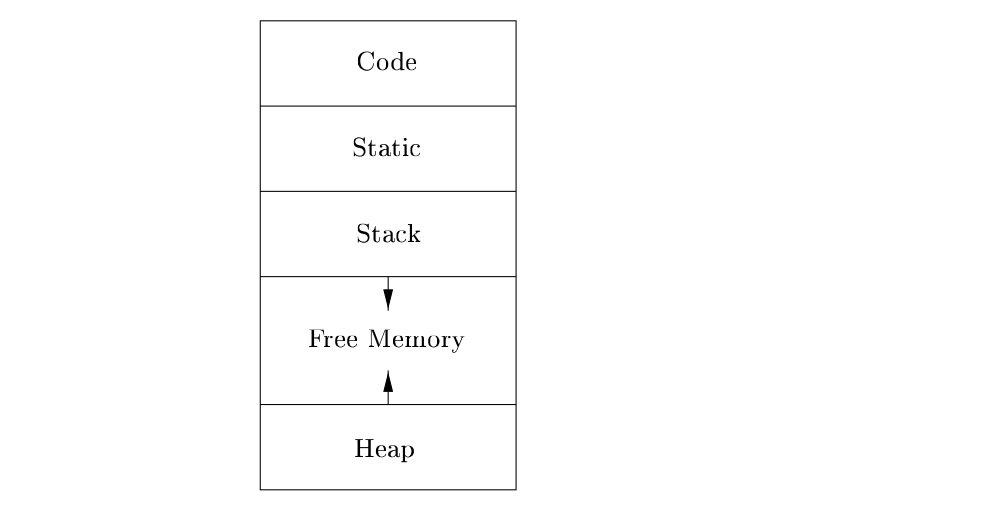
\includegraphics[width=1\textwidth,height=\textheight]{images/memory.png}
\caption{A rough classification of program's
memory segments}
\end{figure}
\end{column}
\end{columns}

\pause

\begin{itemize}
\tightlist
\item
  In practice, the stack grows towards lower
  addresses, the heap towards higher(the diagram
  has it the other way around, but that doesn't
  matter).
\end{itemize}

\pause

\begin{itemize}
\tightlist
\item
  What are all these things ??
\end{itemize}
\end{frame}

\begin{frame}[fragile]{Code and Static segments}
\protect\hypertarget{code-and-static-segments}{}
\begin{itemize}
\tightlist
\item
  \textbf{Code}: Generated target code has a fixed
  size, allowing it to be stored in a statically
  determined area called Code, usually at the low
  end of memory.
\end{itemize}

\pause

\begin{itemize}
\tightlist
\item
  \textbf{Static}: Statically determined data
  objects, such as global constants and data
  generated by the compiler at compile time, can
  be stored in another area called Static.
\end{itemize}

\pause

\begin{minted}[linenos,mathescape,breaklines,breakanywhere,texcomments,escapeinside=||]{c}
const char* s = "Lorem Ipsum something something";
int main(){
  const char* string_arr[] = {"Made", "with", "love", "by", "Delta", "Force"};
  return 0;
}
\end{minted}

All the strings used in the above code segment are
stored in static section, while the instructions
generated for the program will be in code section.
\end{frame}

\begin{frame}{Stack and Stack Allocation}
\protect\hypertarget{stack-and-stack-allocation}{}
\pause

\begin{itemize}
\tightlist
\item
  The stack will store things such as local
  variables, return address from a function call,
  etc.
\end{itemize}
\end{frame}

\begin{frame}[fragile]{Stack and Stack
Allocation(continued)}
\protect\hypertarget{stack-and-stack-allocationcontinued}{}
\begin{columns}[T]
\begin{column}{0.4\textwidth}
\vspace{30pt}

\begin{minted}[linenos,mathescape,breaklines,breakanywhere,texcomments,escapeinside=||]{c}
int main(){
// All of this is
// doing stack allocation
  int a = 10;
  int b = 20;
  int arr[2] = {1,2};
  return 0;
}
\end{minted}
\end{column}

\begin{column}{0.6\textwidth}
\pause

\begin{figure}
\centering
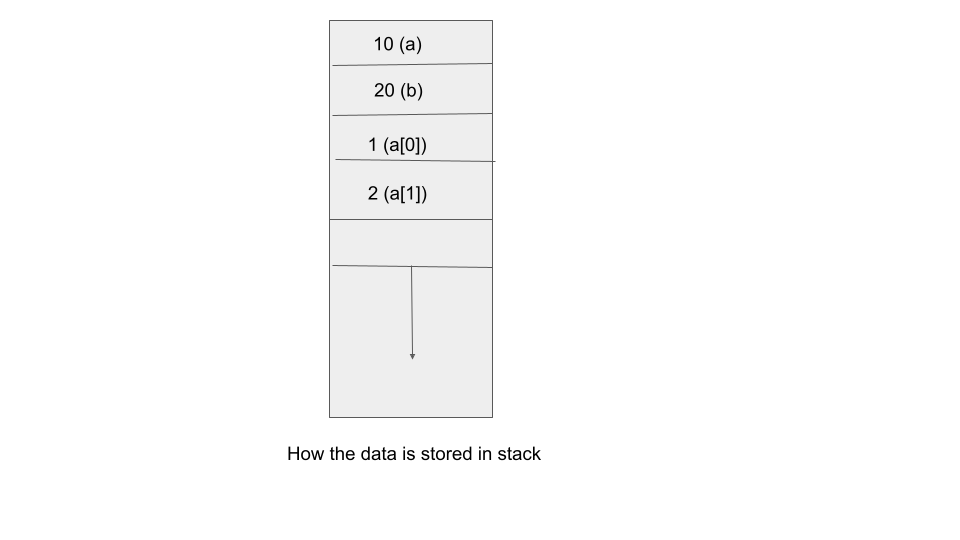
\includegraphics{images/stack_layout.png}
\caption{Stack Layout for above code}
\end{figure}
\end{column}
\end{columns}
\end{frame}

\begin{frame}[fragile]{Heap and Heap Allocation}
\protect\hypertarget{heap-and-heap-allocation}{}
\pause

\begin{itemize}
\tightlist
\item
  Many programming languages allow the programmer
  to allocate and deallocate data under program
  control.
\end{itemize}

\pause

\begin{itemize}
\tightlist
\item
  The heap is used to manage long-lived data.
\end{itemize}

\pause

\begin{itemize}
\tightlist
\item
  Unavoidable when we want to allocate memory
  whose size is known only when the program is
  running(dynamic allocation).
\end{itemize}

\pause

\begin{itemize}
\tightlist
\item
  C/C++ has \texttt{malloc/realloc/free} functions
  for doing heap memory management.
\end{itemize}

\pause

\footnotesize

\begin{minted}[linenos,mathescape,breaklines,breakanywhere,texcomments,escapeinside=||]{c}
int* f(int n){
  return malloc(n*sizeof(int));
}
int main(){
   int n ;
   scanf("%d", &n);
   int *arr = f(n); // arr is heap allocated,returned from call to f
   free(arr); //Since, we're good programmers, we'll free the memory as well.
}
\end{minted}

\normalsize
\end{frame}

\begin{frame}[fragile]{What exactly are
malloc/realloc/free?}
\protect\hypertarget{what-exactly-are-mallocreallocfree}{}
\pause

\begin{itemize}
\tightlist
\item
  \texttt{\textcolor{red}{malloc(x)} }: allocate
  \passthrough{\lstinline!x!} bytes in heap
\end{itemize}

\pause

\begin{itemize}
\tightlist
\item
  \texttt{\textcolor{red}{ realloc(p, x) }}:
  resize previously allocated heap memory
\end{itemize}

\pause

\begin{itemize}
\tightlist
\item
  \texttt{\textcolor{red}{ free(p) } }: return
  heap memory to the operating system
\end{itemize}
\end{frame}

\hypertarget{introduction-to-memory-management}{%
\section{Introduction to Memory
Management}\label{introduction-to-memory-management}}

\begin{frame}{Introduction to Memory Management}
\pause

\begin{itemize}
\tightlist
\item
  Memory management is all about using
  \texttt{heap memory} correctly.
\end{itemize}

\pause

\begin{itemize}
\tightlist
\item
  Stack allocations don't need to be freed;
  they're automatically managed with
  \textbf{scopes} (we'll talk about scopes in the
  next slide).
\end{itemize}

\pause

\begin{itemize}
\tightlist
\item
  If it's done incorrectly, the program can
  \textcolor{red}{crash} or
  \textcolor{red}{slow down}.
\end{itemize}

\pause

\begin{itemize}
\tightlist
\item
  There are different techniques for managing heap
  memory.
\end{itemize}
\end{frame}

\begin{frame}[fragile]{What is this scope thing??}
\protect\hypertarget{what-is-this-scope-thing}{}
\pause

\centering Easier to understand with an example

\pause

\begin{columns}[T]
\begin{column}{0.1\textwidth}
\end{column}

\begin{column}{0.9\textwidth}
\footnotesize

\begin{minted}[linenos,mathescape,breaklines,breakanywhere,texcomments,escapeinside=||]{cpp}
// NOTE: This function won't compile
int f(){ // scope '1 starts
    int a = 10;
    { // scope '2 starts
       int b = 20;
       { // scope '3 stars
           int c = 50;
       } // scope '3 ends
    } // scope '2 ends

    if(a == 10){ // scope '4 starts
      int c = 30;
    } // scope '4 ends
    else { // scope '5 starts
       int c = 90;
    } // scope '5 ends
    return b; // This fails because it's not in scope
} // scope '1 ends
\end{minted}

\normalsize
\end{column}
\end{columns}
\end{frame}

\begin{frame}{What is this scope thing??
(continued)}
\protect\hypertarget{what-is-this-scope-thing-continued}{}
\begin{figure}
\centering
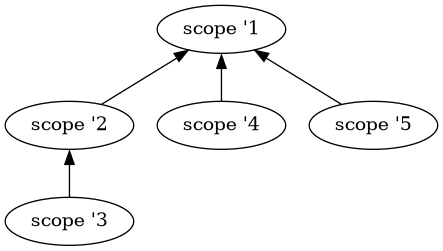
\includegraphics{images/scope.png}
\caption{Pictorial representation of scope
heirarchy}
\end{figure}
\end{frame}

\begin{frame}{Why should I care about freeing
memory? Is it really a problem?}
\protect\hypertarget{why-should-i-care-about-freeing-memory-is-it-really-a-problem}{}
\pause

\begin{itemize}
\tightlist
\item
  If your system has infinite memory, you don't
  need to worry. However, since memory is finite,
  you must take care. \pause
\item
  If one program uses up all the memory, other
  programs that require memory won't be able to
  function properly. \pause
\item
  Your program may \textcolor{red}{crash} if it
  requests more memory than the operating system
  can provide. \pause
\item
  \textcolor{red}{Memory leaks} can have a
  significant impact on long-running programs such
  as \texttt{web servers, editors, and IDEs}.
\end{itemize}

\pause

\begin{block}{Important terminology}
\protect\hypertarget{important-terminology}{}
\begin{itemize}
\tightlist
\item
  \textbf{\textcolor{red}{Memory Leak}}: It
  happens when you ask the operating system for
  memory but don't return it back.
\end{itemize}
\end{block}
\end{frame}

\hypertarget{ways-to-manage-memory}{%
\section{Ways to manage
memory}\label{ways-to-manage-memory}}

\begin{frame}{Ways to manage memory}
We have two ways to do memory management.

\pause

\begin{itemize}
\tightlist
\item
  \textbf{Manual Memory Management} : Languages
  such as C, C++, Rust, etc have this
\end{itemize}

\pause

\begin{itemize}
\tightlist
\item
  \textbf{Automatic Memory Management}: Languages
  such as Python, Java, Go, JavaScript, Swift, etc
  have this.
\end{itemize}
\end{frame}

\hypertarget{manual-memory-management}{%
\section{Manual Memory
Management}\label{manual-memory-management}}

\begin{frame}[fragile]{Scenarios where you can go
wrong}
\protect\hypertarget{scenarios-where-you-can-go-wrong}{}
\begin{columns}[T]
\begin{column}{0.48\textwidth}
\scriptsize

\begin{minted}[linenos,mathescape,breaklines,breakanywhere,texcomments,escapeinside=||]{cpp}
// NOTE: this is a dumb example to show where things can go wrong,
// I don't actually write code like this
int* allocate_and_throw_exn(int n){
   int *arr = malloc(n*sizeof(int));
   if (n < 10){
       throw runtime_error("n < 10");
   }
   return arr;
}
int main(){
    try {
        auto *arr = allocate_and_throw_exn(2);
        free(arr);
    } catch(const std::runtime_error &e){
        cout << "Error:" <<e.what() << endl;
    }
}
\end{minted}

\normalsize
\end{column}

\begin{column}{0.48\textwidth}
\vspace{30pt}

\pause

\begin{figure}
\centering
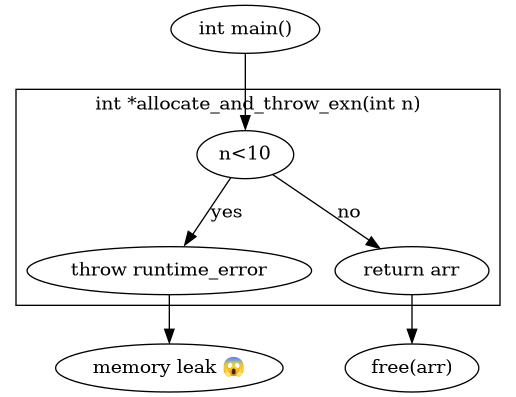
\includegraphics[width=1.15\textwidth,height=\textheight]{images/mem_management_leak_scenario1.png}
\caption{Flow for the leaking code}
\end{figure}
\end{column}
\end{columns}
\end{frame}

\begin{frame}{Scenarios where you can go wrong}
\protect\hypertarget{scenarios-where-you-can-go-wrong-1}{}
\begin{figure}
\centering
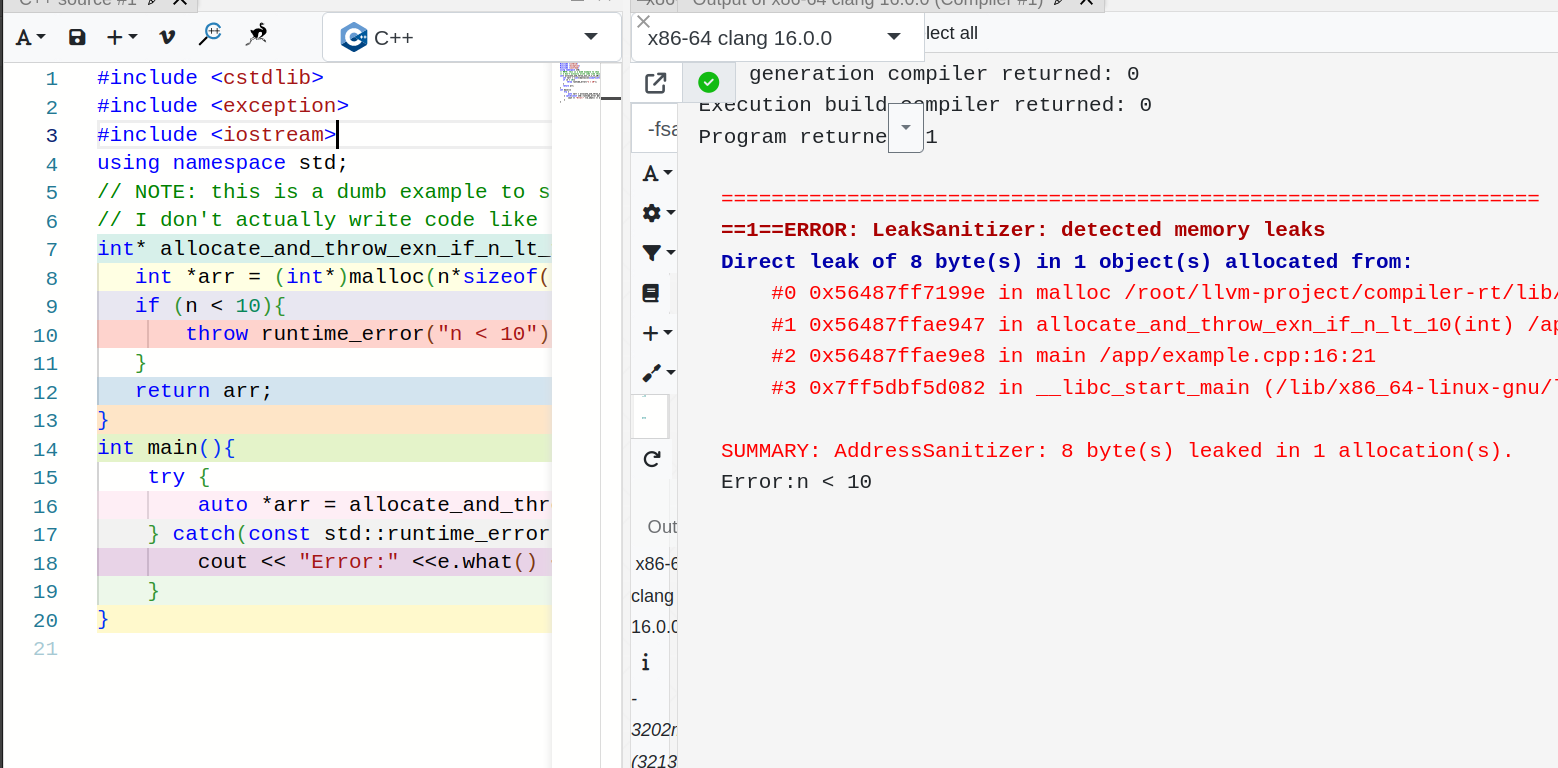
\includegraphics[width=1\textwidth,height=\textheight]{images/./leak_detected.png}
\caption{Memory Leak Detected by address
sanitizer}
\end{figure}
\end{frame}

\begin{frame}{How to fix it??}
\protect\hypertarget{how-to-fix-it}{}
\pause

\begin{itemize}
\tightlist
\item
  \textcolor{red}{DON'T WRITE DUMB CODE LIKE I DID}
\end{itemize}

\pause

\begin{itemize}
\tightlist
\item
  More high level language(than C) like C++, Rust
  provide us with smart ways to manage memory
\end{itemize}

\pause

\begin{itemize}
\tightlist
\item
  They come built-in with smart pointer types like
  \texttt{unique\textunderscore ptr} (C++)
\end{itemize}
\end{frame}

\begin{frame}[fragile]{Fixing the code with smart
pointer}
\protect\hypertarget{fixing-the-code-with-smart-pointer}{}
\begin{columns}[T]
\begin{column}{0.48\textwidth}
\scriptsize

\begin{minted}[linenos,mathescape,breaklines,breakanywhere,texcomments,escapeinside=||]{cpp}
# \textcolor{red}{LEAKING CODE}
int* allocate_and_throw_exn(int n){
   int *arr = malloc(n*sizeof(int));
   if (n < 10){
       throw runtime_error("n < 10");
   }
   return arr;
}
int main(){
    try {
        auto *arr = allocate_and_throw_exn(2);
        free(arr);
    } catch(const std::runtime_error &e){
        cout << "Error:" <<e.what() << endl;
    }
}
\end{minted}

\normalsize

\pause
\end{column}

\begin{column}{0.48\textwidth}
\scriptsize

\begin{minted}[linenos,mathescape,breaklines,breakanywhere,texcomments,escapeinside=||]{cpp}
# \textcolor{red}{FIXED CODE}
std::unique_ptr<int[]> allocate_and_throw_exn(int n){
   auto arr = std::unique_ptr<int[]>(new int[n]);
   if (n < 10){
       throw runtime_error("n < 10");
   }
   return arr;
}
int main(){
    try {
        auto arr = allocate_and_throw_exn(2);
    } catch(const std::runtime_error &e){
        cout << "Error:" <<e.what() << endl;
    }
}
\end{minted}

\normalsize
\end{column}
\end{columns}

\pause
\begin{center}

\textbf{\textcolor{red}{What the hell just happened??}}
\end{center}
\end{frame}

\begin{frame}{How do smart pointers work?}
\protect\hypertarget{how-do-smart-pointers-work}{}
\pause

\begin{itemize}
\tightlist
\item
  Uses \textbf{scope} to track lifetime of a
  pointer(scopes mentioned in
  \protect\hyperlink{what-is-this-scope-thing}{previous
  section})
\end{itemize}

\pause

\begin{itemize}
\tightlist
\item
  C++ uses \texttt{destructors} to run code when
  an object goes out of scope. (due to
  \textcolor{red}{RAII} in C++)
\end{itemize}
\end{frame}

\begin{frame}{How do smart pointers work?
(continued)}
\protect\hypertarget{how-do-smart-pointers-work-continued}{}
\begin{block}{What is RAII in C++?}
\protect\hypertarget{what-is-raii-in-c}{}
\begin{figure}
\centering
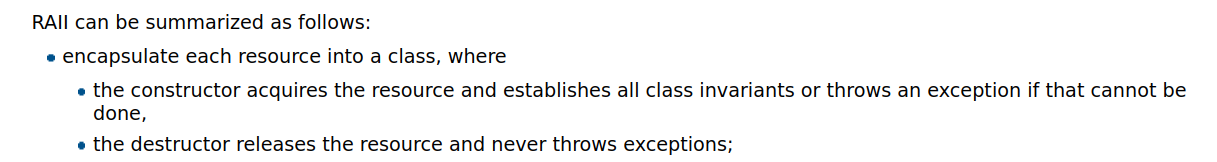
\includegraphics{images/raii.png}
\caption{RAII}
\end{figure}
\end{block}
\end{frame}

\begin{frame}{Destructors In Action}
\protect\hypertarget{destructors-in-action}{}
\begin{figure}
\centering
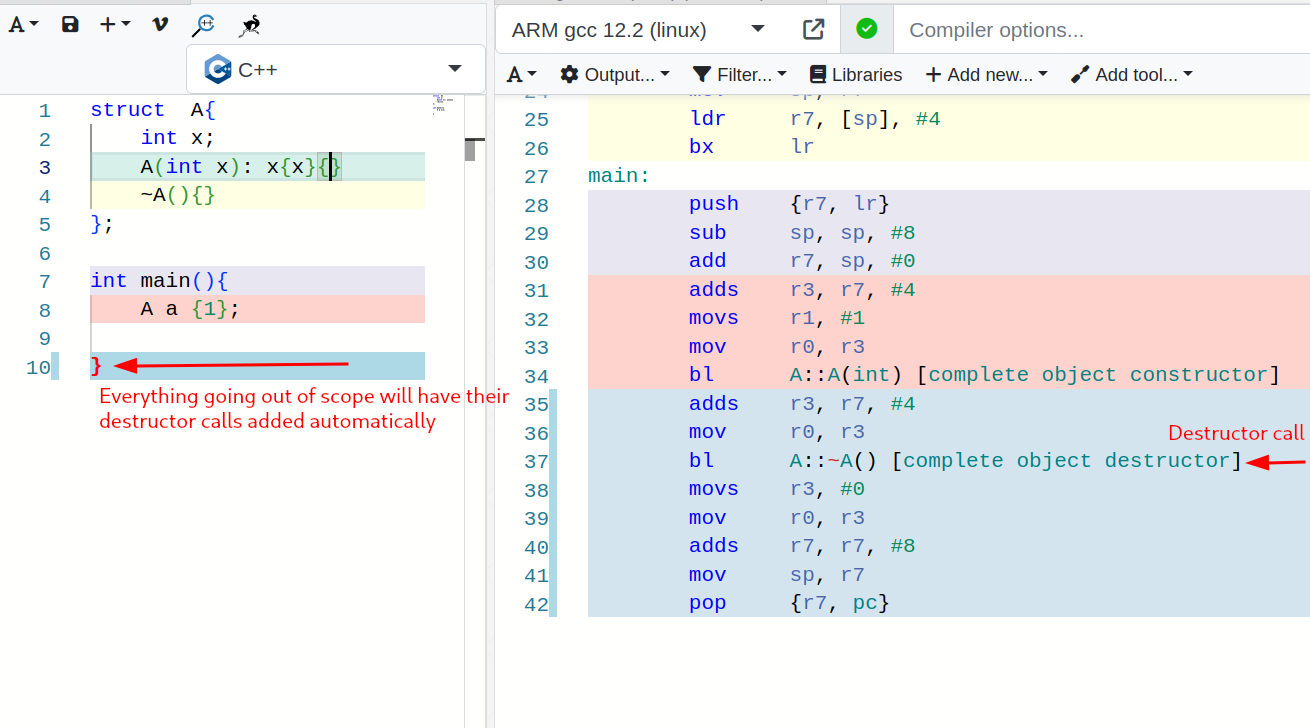
\includegraphics{images/./destructor.png}
\caption{Destructor call added automatically}
\end{figure}
\end{frame}

\begin{frame}[fragile]{Let's make our own
unique\_ptr}
\protect\hypertarget{lets-make-our-own-unique_ptr}{}
\pause

\begin{columns}[T]
\begin{column}{0.48\textwidth}
\scriptsize

\begin{minted}[linenos,mathescape,breaklines,breakanywhere,texcomments,escapeinside=||]{cpp}
#include <iostream>
using namespace std;
class int_ptr{
    int* x ;
public:
    int_ptr(int x): x{new int(x)}{}
    ~int_ptr(){
        delete x;
    }
    int& operator*(){
        return *x;
    }
};
int main(){
    int_ptr one(1);
    cout << *one << endl;
}
\end{minted}

\normalsize
\end{column}

\begin{column}{0.48\textwidth}
\vspace{30pt}

\begin{figure}
\centering
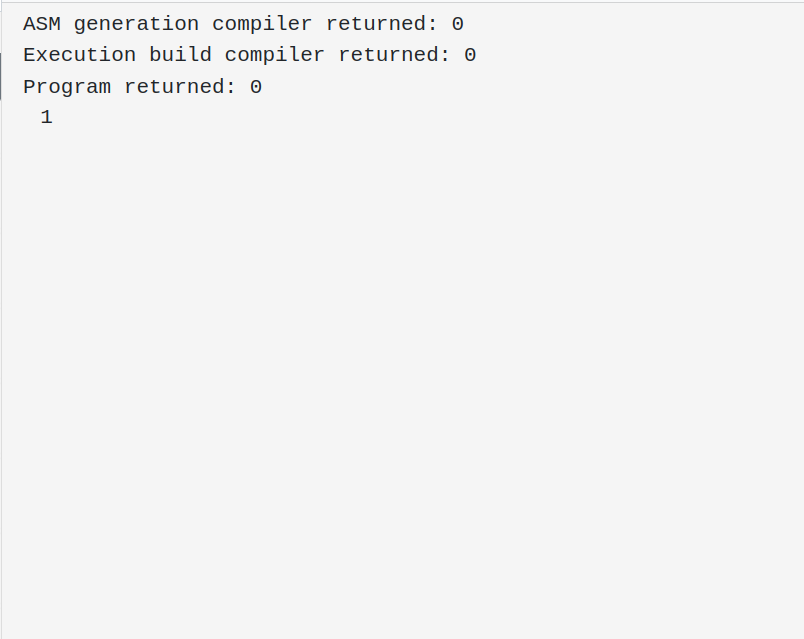
\includegraphics{images/./int_ptr_working.png}
\caption{int\_ptr working without any leaks}
\end{figure}
\end{column}
\end{columns}
\end{frame}

\begin{frame}{Is unique\_ptr the only smart
pointer??}
\protect\hypertarget{is-unique_ptr-the-only-smart-pointer}{}
\pause
\huge

\centering\textbf{\textcolor{red}{ NO }}
\normalsize
\end{frame}

\begin{frame}{Isn't unique\_ptr perfect already?
Why would I need anything else?}
\protect\hypertarget{isnt-unique_ptr-perfect-already-why-would-i-need-anything-else}{}
\pause

\begin{itemize}
\tightlist
\item
  Problem with \texttt{unique\textunderscore ptr}
  is that it can have only one owner.
\end{itemize}

\pause

\begin{block}{Case in Point}
\protect\hypertarget{case-in-point}{}
\begin{itemize}
\tightlist
\item
  A \texttt{unix file descriptor}
\end{itemize}

\pause

\begin{itemize}
\tightlist
\item
  A file descriptor can have multiple owners. It
  should only be freed when all the owners go out
  of scope.
\end{itemize}
\end{block}
\end{frame}

\begin{frame}{File Descriptors Example and what's
the problem}
\protect\hypertarget{file-descriptors-example-and-whats-the-problem}{}
\pause

\centering \textcolor{red}{DISCLAIMER:} The code
that I'm about to show is cursed and no one should
model a file descriptor like this

\pause

\centering But, we'll do it still(for the purpose
of this talk)
\end{frame}

\begin{frame}{File Descriptors (continued)}
\protect\hypertarget{file-descriptors-continued}{}
\pause

\begin{figure}
\centering
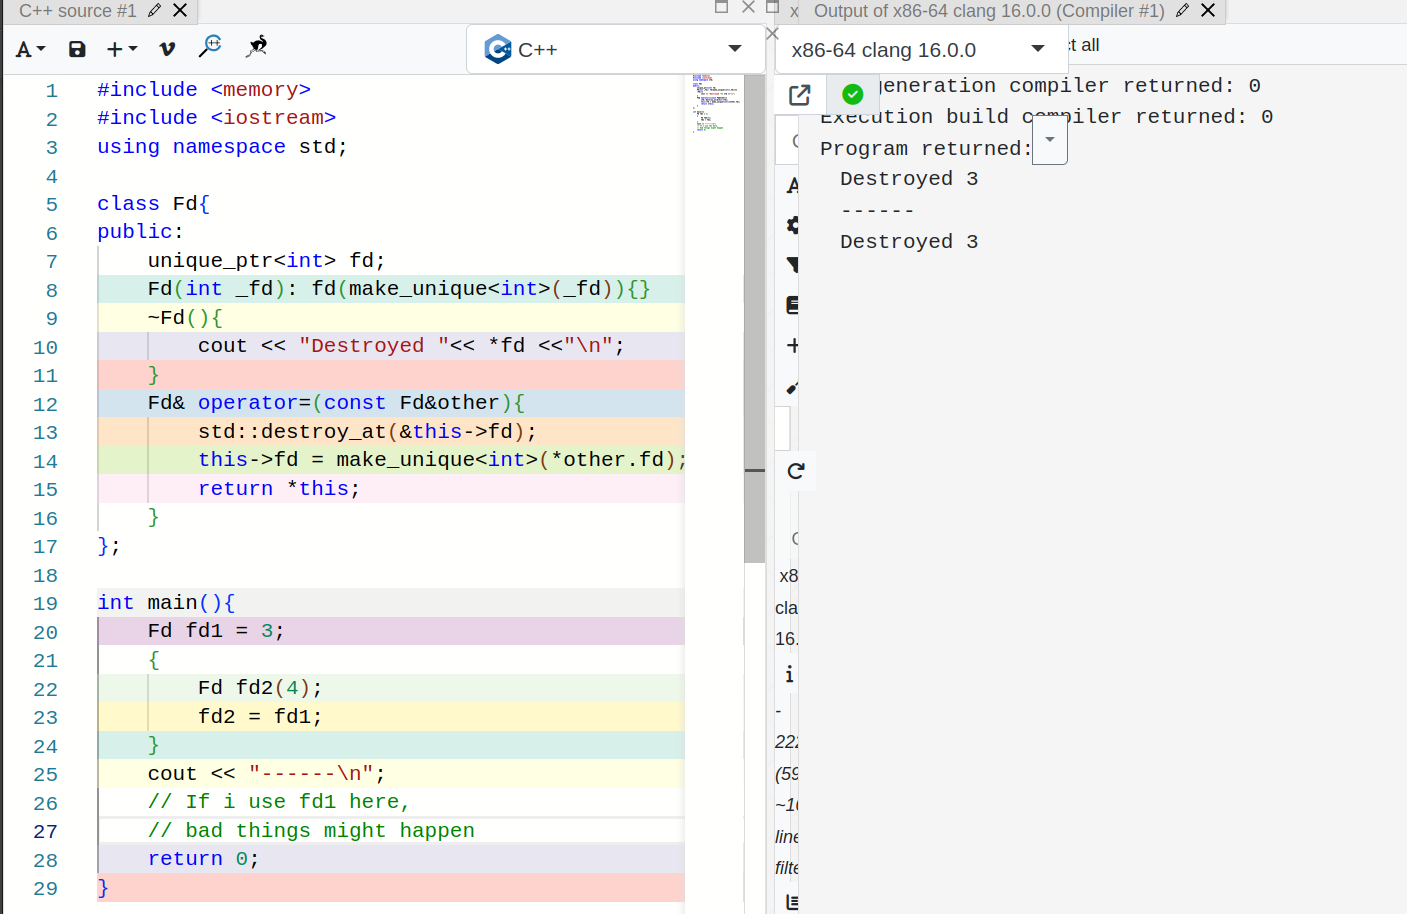
\includegraphics[width=0.9\textwidth,height=\textheight]{images/./fd.png}
\caption{File Descriptor with unique\_ptr}
\end{figure}

\pause

\vspace{-10pt}

\centering {\textcolor{red}{\textbf{Not possible to model this correctly }}}
\end{frame}

\begin{frame}{Another classic example (why only
unique\_ptr isn't enough?)}
\protect\hypertarget{another-classic-example-why-only-unique_ptr-isnt-enough}{}
\begin{itemize}
\tightlist
\item
  \textcolor{red}{SPMC(Single Producer Multiple Consumer) }
  and
  \textcolor{red}{MPMC(Multiple Producer Multiple Consumer)}
  problem
\end{itemize}

\pause

\begin{figure}
\centering
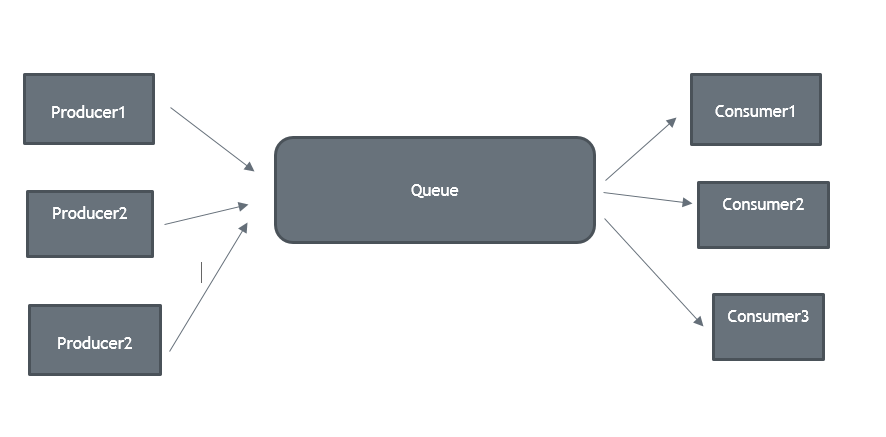
\includegraphics[width=0.8\textwidth,height=\textheight]{images/mpmc.png}
\caption{MPMC queue}
\end{figure}

\pause

\begin{itemize}
\tightlist
\item
  Requires multiple owners for producer end as
  well as the consumer end
\end{itemize}
\end{frame}

\hypertarget{introduction-to-automatic-memory-management}{%
\section{Introduction to Automatic Memory
Management}\label{introduction-to-automatic-memory-management}}

\begin{frame}{Introduction to Automatic Memory
Management}
\pause

\begin{itemize}
\tightlist
\item
  The programming language you're using is
  responsible for memory management. The language
  runtime handles everything.
\end{itemize}

\pause

\begin{itemize}
\tightlist
\item
  Programmer doesn't have the mental burden of
  dealing with memory.
\end{itemize}

\pause

\begin{itemize}
\tightlist
\item
  All the allocation/deallocation calls are hidden
  from the programmer.
\end{itemize}

\pause

\begin{block}{\centering IMPORTANT TERMINOLOGY}
\protect\hypertarget{important-terminology-1}{}
\pause

\begin{center}
\textcolor{red}{Data that cannot be referenced is generally known as \textbf{garbage}}
\end{center}
\pause
\end{block}

\begin{block}{\centering Two techniques used
primarily}
\protect\hypertarget{two-techniques-used-primarily}{}
\pause

\begin{itemize}
\tightlist
\item
  We catch the transitions as
  \texttt{reachable}(in-scope) objects turn
  \texttt{unreachable}(out-of-scope).
  \pause Example:
  \textcolor{red}{Reference Counting} based memory
  management in Python, Swift,etc., C++
  shared\_ptr, Rust's Rc and Arc types
\end{itemize}

\pause

\begin{itemize}
\tightlist
\item
  We periodically locate all the
  \texttt{reachable} objects and then infer that
  all the other objects are \texttt{unreachable}.
  \pause Example:
  \textcolor{red}{Trace Based Garbage Collection}
  such as mark and sweep garbage collector used in
  language like Java, JavaScript, etc.
\end{itemize}
\end{block}
\end{frame}

\hypertarget{reference-counting}{%
\section{Reference
Counting}\label{reference-counting}}

\begin{frame}{Reference Counting}
\pause

\begin{itemize}
\tightlist
\item
  All the transitions from reachable to
  unreachable are caught immediately. \pause
\end{itemize}

\begin{block}{Backed by simple rules}
\protect\hypertarget{backed-by-simple-rules}{}
\pause

\begin{itemize}
\tightlist
\item
  Every allocated pointer has a
  \textcolor{red}{reference count} associated with
  it \pause
\item
  Every copy leads to reference count increment.
  \pause
\item
  Every time a reference of the pointer goes out
  of scope, reference count is decremented by
  \(1\). \pause
\item
  When the reference count goes to \(0\), it is
  safe to \texttt{free} the object.
\end{itemize}
\end{block}
\end{frame}

\begin{frame}{C++'s shared\_ptr type}
\protect\hypertarget{cs-shared_ptr-type}{}
\pause

\begin{itemize}
\tightlist
\item
  It is a \texttt{reference-counted pointer},
  manages the \texttt{reference count} elegantly
  with assignment operator overload, copy
  constructor overload, destructors, etc.
\end{itemize}
\end{frame}

\begin{frame}{Let's solve our file descriptor
issue}
\protect\hypertarget{lets-solve-our-file-descriptor-issue}{}
\pause

\begin{figure}
\centering
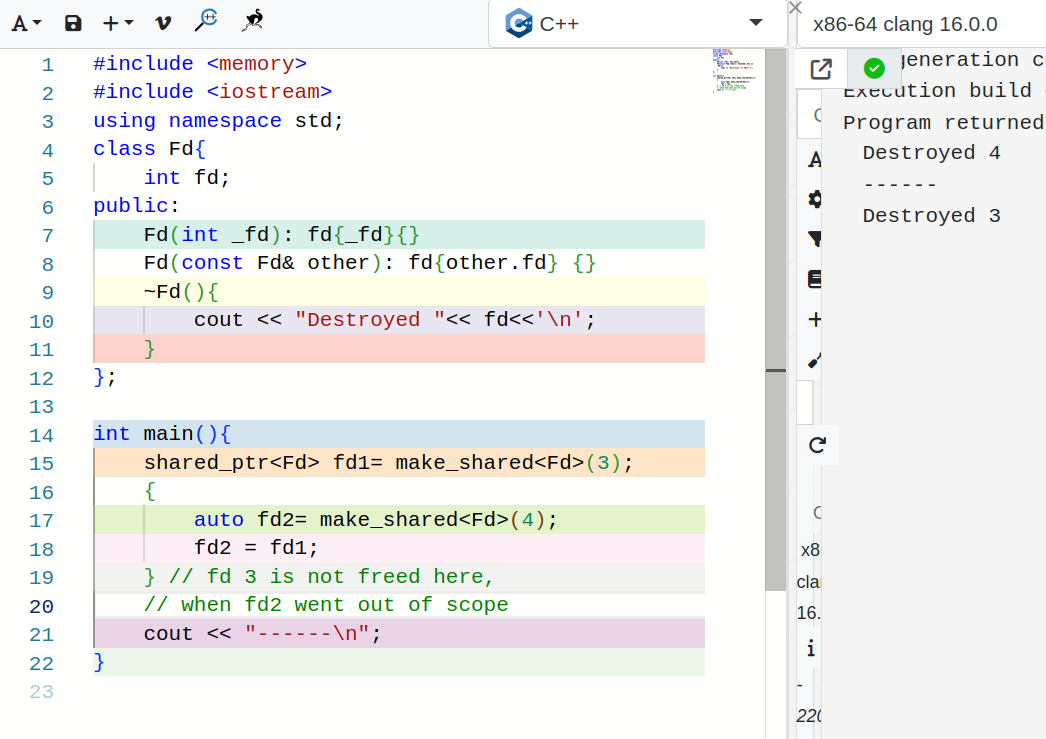
\includegraphics[width=0.85\textwidth,height=\textheight]{images/fd_with_rc.png}
\caption{File Descriptor with shared\_pointer}
\end{figure}
\end{frame}

\hypertarget{trace-based-garbage-collection}{%
\section{Trace Based Garbage
Collection}\label{trace-based-garbage-collection}}

\begin{frame}{Trace Based Garbage Collection}
\pause

\begin{itemize}
\tightlist
\item
  Periodically locates all the \texttt{reachable}
  objects and then infers that all the other
  objects are \texttt{unreachable}
\end{itemize}

\pause

\begin{itemize}
\tightlist
\item
  A pointer is reachable
  \(\textcolor{red}{\Rightarrow }\) There's a root
  somewhere(in stack, register, static, etc.) from
  where we can transitively access the pointer.
\end{itemize}
\end{frame}

\begin{frame}[fragile]{What's a root?}
\protect\hypertarget{whats-a-root}{}
\pause

Think of them as root nodes of a graph, something
that you have direct access to.

\pause

A \texttt{GC} will treat all the stack variables,
registers, static section, as roots.

\text

\begin{columns}[T]
\begin{column}{0.48\textwidth}
\pause

\scriptsize

\begin{minted}[linenos,mathescape,breaklines,breakanywhere,texcomments,escapeinside=||]{ocaml}
type baz = {
    x: int;
    y: int
}
type bar = {
    a:  int;
    b:  baz
}
type foo = {
    field1 : bar;
    field2: int
}
let foo_instance: foo = {
    field1 = {
        a  = 10;
        b = { x= 2 ;y= 5; };
    };
    field2= 5;
}
\end{minted}

\normalsize
\end{column}

\begin{column}{0.48\textwidth}
\pause

\begin{figure}
\centering
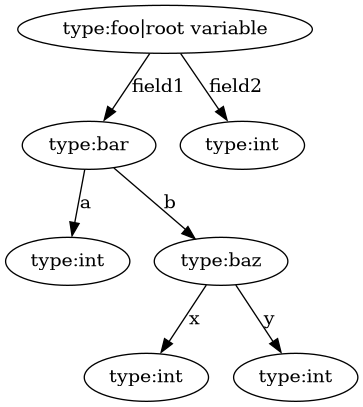
\includegraphics[width=0.8\textwidth,height=\textheight]{images/object_graph.png}
\caption{foo\_instance variable as a graph}
\end{figure}
\end{column}
\end{columns}
\end{frame}

\begin{frame}{Root finding}
\protect\hypertarget{root-finding}{}
\pause

\begin{itemize}
\tightlist
\item
  \textcolor{red}{It involves many intricate details, which took me quite a while to understand.}
\end{itemize}

\pause

\begin{itemize}
\tightlist
\item
  You'd probably want to design a
  \texttt{precise-collector} if you're building
  your own language.
  \pause \textcolor{red}{Precise Collector} is
  when GC knows about root objects: where they're
  placed on stack,their size,lifetime etc.
  \pause Most popular language runtimes use
  precise garbage collectors: Python, PyPy,
  JVM(Java), .NET(C\#), Lua, V8(JavaScript)
  ,SpiderMonkey(JavaScript) and a lot of others.
\end{itemize}

\pause

\begin{itemize}
\tightlist
\item
  Conservative collection does not know about
  types of traced GC objects. \pause It'll assume
  everything that's present in the stack, static
  and register are pointers and it'll follow it.
  \pause They are inherently unsafe.
  \pause Example: Boehm-Demers-Weiser conservative
  C/C++ Garbage Collector
\end{itemize}
\end{frame}

\begin{frame}{Tracing GC Algorithms}
\protect\hypertarget{tracing-gc-algorithms}{}
\pause

All trace-based algorithms compute the set of
reachable objects and then take the complement of
this set. Memory is therefore recycled as follows:

\pause

\begin{enumerate}
\tightlist
\item
  The program or mutator runs and makes allocation
  requests. \pause
\item
  The garbage collector discovers reachability by
  tracing. \pause
\item
  The garbage collector reclaims the storage for
  unreachable objects.
\end{enumerate}

\pause

\begin{block}{\centering Tracing Based GC
Algorithms}
\protect\hypertarget{tracing-based-gc-algorithms}{}
\pause

\begin{itemize}
\item
  Copying Collector
\item
  Mark and Sweep Collector
\end{itemize}
\end{block}
\end{frame}

\begin{frame}{Copying Collector}
\protect\hypertarget{copying-collector}{}
\pause

\begin{itemize}
\tightlist
\item
  \textcolor{red}{Copying Collector} partitions
  memory into two semispaces, A and B. \pause
\item
  All the allocations are performed in one
  semispace until it fills up. \pause
\item
  The garbage collector then copies reachable
  objects to the other space. \pause
\item
  Roles of the semispaces are reversed when
  garbage collection is complete. \pause
\item
  While all this is happening, the whole program
  is stopped. (This is why it's called a
  stop-the-world algorithm)
\end{itemize}
\end{frame}

\begin{frame}{Copying Collector (A visual
representation)}
\protect\hypertarget{copying-collector-a-visual-representation}{}
\pause

\begin{columns}[T]
\begin{column}{0.48\textwidth}
\begin{figure}
\centering
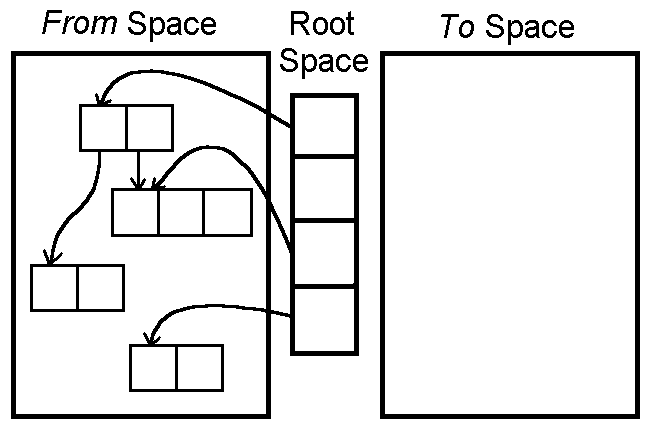
\includegraphics[width=1\textwidth,height=\textheight]{images/copying_collector_before.png}
\caption{Before GC}
\end{figure}
\end{column}

\pause

\begin{column}{0.48\textwidth}
\begin{figure}
\centering
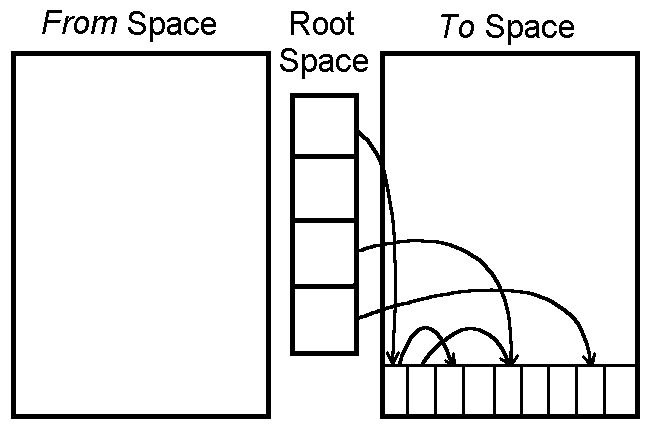
\includegraphics[width=1\textwidth,height=\textheight]{images/copying_collector_after.png}
\caption{After GC}
\end{figure}
\end{column}
\end{columns}
\end{frame}

\begin{frame}{Mark and Sweep}
\protect\hypertarget{mark-and-sweep}{}
\pause

\centering \textbf{\textcolor{red}{Some terminology first}}

\pause

In a \texttt{mark-and-sweep} gc, An object may be
in one of the 4 states: Free(Blue),
Unreached(White), Unscanned(Gray), Scanned(Black)

\pause

It is also a stop-the-world algorithm.

\pause \textcolor{red}{Mark}
\rightarrow responsible for marking reachable
objects \texttt{Black}

\pause \textcolor{red}{Sweep}
\rightarrow responsible for freeing all the
unreachable( \texttt{White} ) objects.
\end{frame}

\begin{frame}{Mark and Sweep(continued)}
\protect\hypertarget{mark-and-sweepcontinued}{}
\begin{figure}
\centering
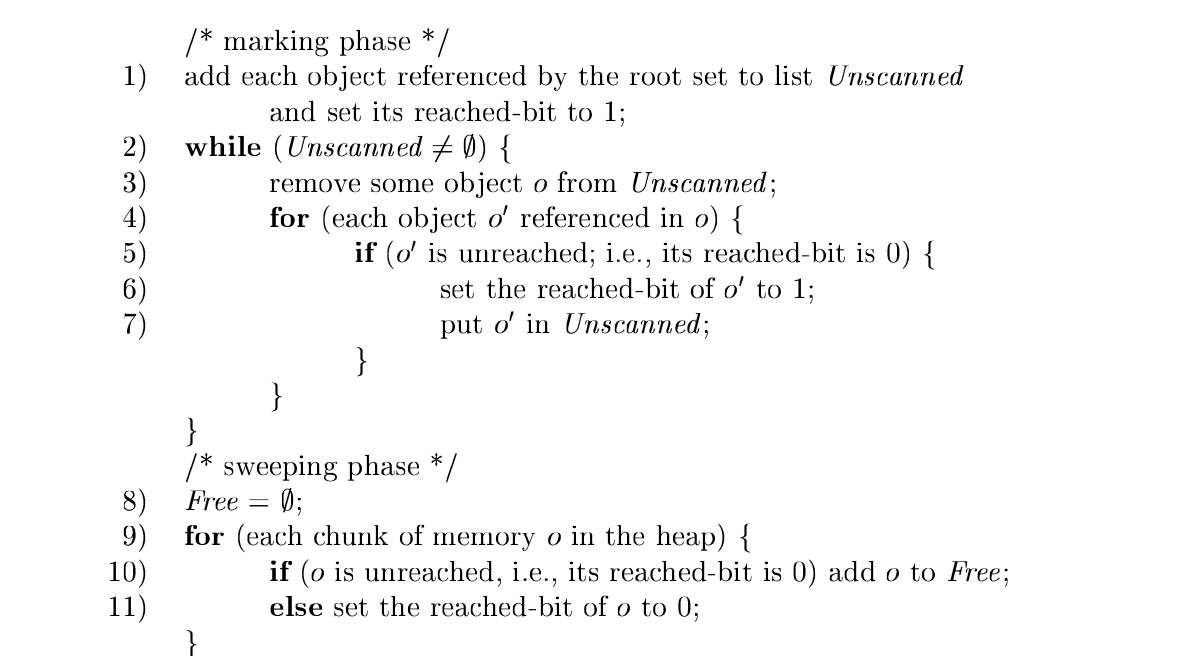
\includegraphics{images/mark_and_sweep.png}
\caption{Basic Mark and Sweep}
\end{figure}
\end{frame}

\hypertarget{which-is-better-automatic-memory-management-or-manual-management}{%
\section{Which is better ? (Automatic Memory
Management or Manual
Management)}\label{which-is-better-automatic-memory-management-or-manual-management}}

\begin{frame}{Which is better ? (Automatic Memory
Management or Manual Management)}
\pause

\huge

\centering \textbf{\textcolor{red}{DEPENDS}}
\normalsize
\end{frame}

\begin{frame}{Case against Manual Memory
Management}
\protect\hypertarget{case-against-manual-memory-management}{}
\begin{figure}
\centering
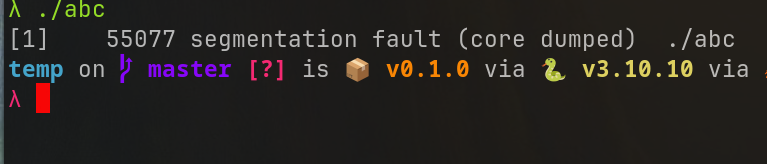
\includegraphics{images/seg_fault.png}
\caption{Segmentation Faults}
\end{figure}
\end{frame}

\begin{frame}{Case against Manual Memory
Management(continued)}
\protect\hypertarget{case-against-manual-memory-managementcontinued}{}
\begin{figure}
\centering
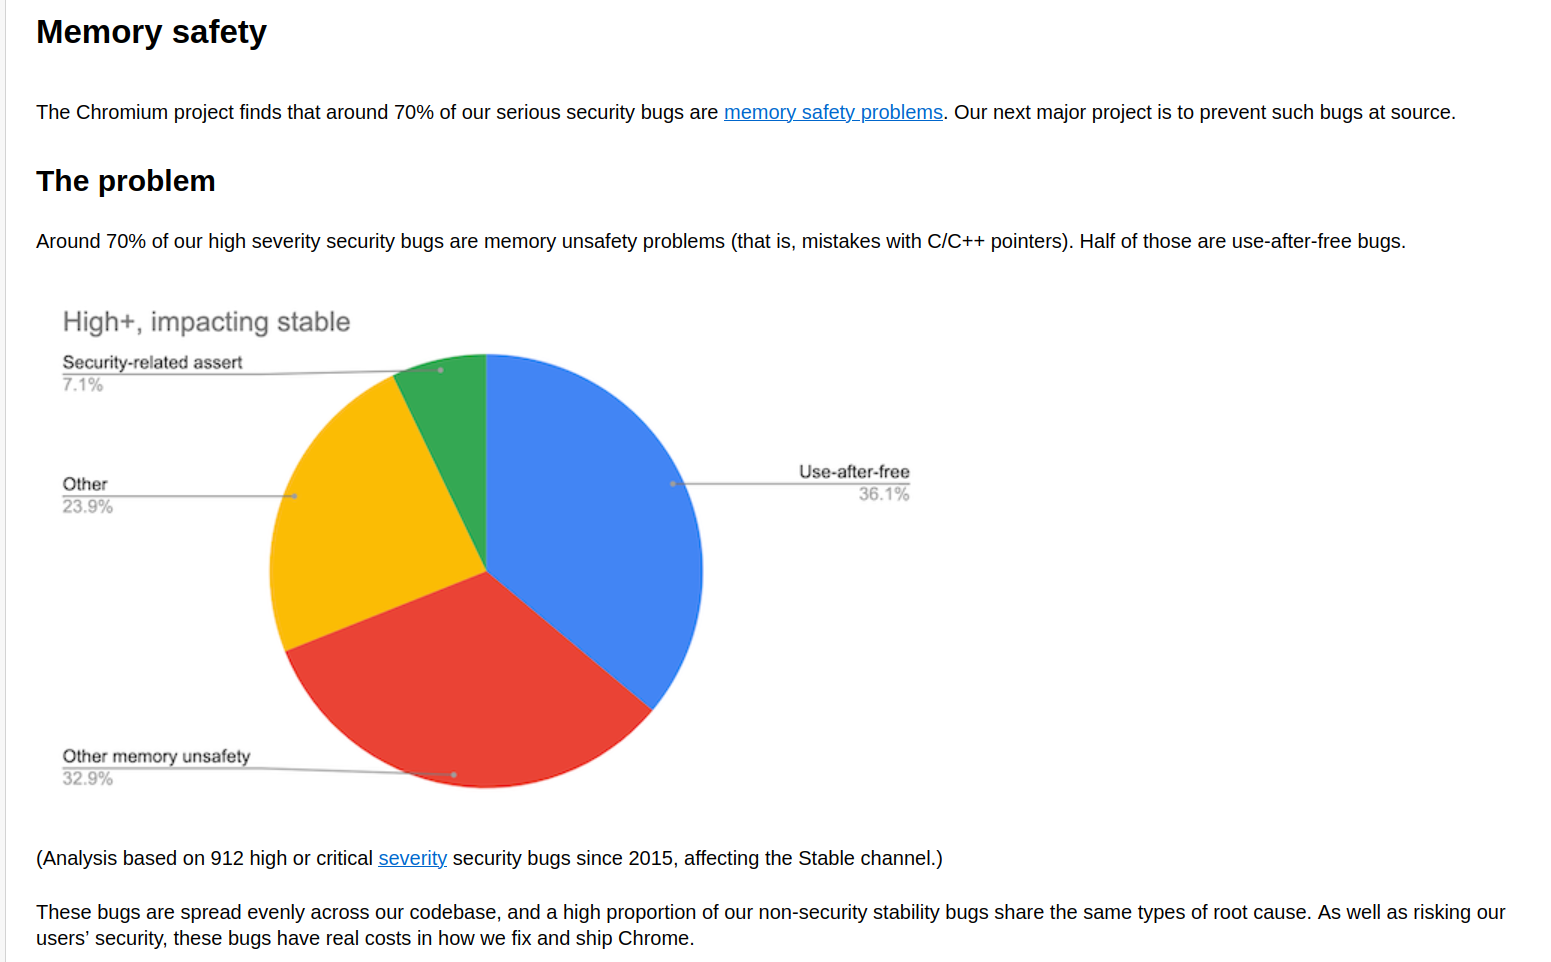
\includegraphics{images/chrome.png}
\caption{Use After Free}
\end{figure}
\end{frame}

\begin{frame}{Case against Automatic Memory
Management}
\protect\hypertarget{case-against-automatic-memory-management}{}
\begin{figure}
\centering
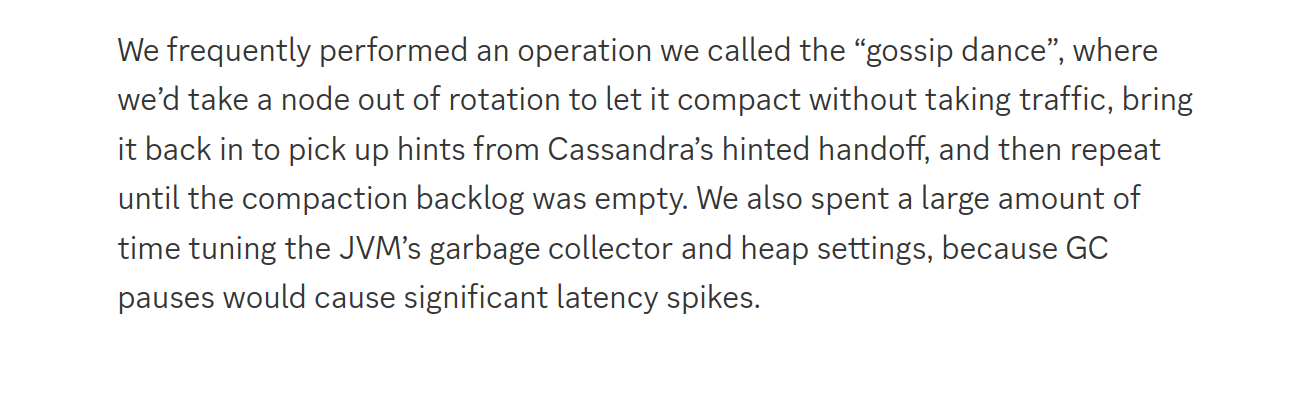
\includegraphics{images/discord_troubles.png}
\caption{Discord Troubles(from a recent Discord
Engineering Blog)}
\end{figure}

\pause

\begin{itemize}
\tightlist
\item
  Similar GC issues encountered by many tech
  giants
\end{itemize}
\end{frame}

\hypertarget{advanced-topics-in-memory-management}{%
\section{Advanced Topics in Memory
Management}\label{advanced-topics-in-memory-management}}

\begin{frame}{Advanced Topics in Memory
Management}
\pause

\begin{itemize}
\tightlist
\item
  Advanced type system like in Rust, which help
  with memory safety
\end{itemize}

\pause

\begin{itemize}
\tightlist
\item
  Incremental GC
\end{itemize}

\pause

\begin{itemize}
\tightlist
\item
  Parallel and Concurrent GC
\end{itemize}

\pause

\begin{itemize}
\tightlist
\item
  Generational GC
\end{itemize}

\pause

\begin{itemize}
\tightlist
\item
  Reducing GC pauses
\end{itemize}
\end{frame}

\hypertarget{references}{%
\section{References}\label{references}}

\begin{frame}{References}
\begin{itemize}
\tightlist
\item
  \url{https://rebelsky.cs.grinnell.edu/Courses/CS302/99S/Presentations/GC/}
\item
  \url{https://discord.com/blog/how-discord-stores-trillions-of-messages}
\item
  \url{https://gchandbook.org/}
\item
  Compilers: Principles, Techniques, and Tools by
  Alfred V. Aho, Monica S. Lam, Ravi Sethi, and
  Jeffrey D. Ullman
\item
  \href{https://en.cppreference.com/w/}{cppreference}
\end{itemize}
\end{frame}

\end{document}
